\documentclass[12 pt]{exam}
\usepackage{graphicx, enumitem, amsmath, amssymb}
\graphicspath{ {./images/} }
\usepackage{tikz, pgfplots}
\usetikzlibrary{shapes,arrows}
%\usepackage{Minion Pro}
\printanswers

\title{1.9 Price Elasticity - Practice Problems (Answers)}
\author{Ryan Safner}
\date{ECON 306 - Spring 2020}

\begin{document}

\maketitle

The demand for monthly cell phone plans is given by:

$$q_D =  50-0.5p$$

\begin{questions}

\question  Write the *inverse* demand function.

\begin{solution}

\begin{align*}
	q_D&=50-0.5p\\
	q_D+0.5p&=50\\
	0.5p&=50-q_D\\
	p&=100-2q_D\\
\end{align*}

The choke price is \$100 and the slope is $-2$.

\end{solution}

\question Calculate the price elasticity of demand when the price is \$10. Is this relatively elastic or inelastic?

\begin{solution}

First we need to find $q_D$ at \$10. 

\begin{align*}
	q_D&=50-0.5(10)\\
	q_D&=50-5\\
	q_D&=45\\
\end{align*}

	Now we have the three ingredients to calculate elasticity at \$10:
	 
\begin{align*}
	\epsilon_D &=\frac{1}{slope} \times \frac{p}{q_D}	\\
	\epsilon_D &=\frac{1}{-2} \times \frac{10}{45}	\\
	\epsilon_D &=-0.5 \times 0.22\\
	\epsilon_D &=-0.11\\
\end{align*}

The demand is relatively inelastic, as $|\epsilon_D|<1$ 

\end{solution}

\question Calculate the price elasticity of demand when the price is \$70. Is this relatively elastic or inelastic?

\begin{solution}
First we need to find $q_D$ at \$70. 
	\begin{align*}
	q_D&=50-0.5(70)\\
	q_D&=50-35\\
	q_D&=15\\
	\end{align*}
	We already have the slope (since the demand is a straight line), so now we can simply plug into the elasticity formula:
		\begin{align*}
	\epsilon_D &=\frac{1}{slope} \times \frac{p}{q_D}	\\
	\epsilon_D &=\frac{1}{-2} \times \frac{70}{15}\\
	\epsilon_D &=-0.5 \times 4.67\\
	\epsilon_D &\approx -2.33\\
	\end{align*}
The demand is relatively elastic, as $|\epsilon_D|>1$

\end{solution}

\question At what price is demand unit elastic $(\epsilon=-1)$?

\begin{solution}

\begin{align*}
		\epsilon_D &=\frac{1}{slope} \times \frac{p}{q_D} & & \text{Formula for elasticity}\\
			-1&=-0.5 \times \frac{p}{q_D} & & \text{Set } \epsilon_D \text{ equal to }-1\\
			-1&=-0.5 \times \frac{p}{(50-0.5p)} & & \text{Plug in demand function for } q_D\\
			-1(50-0.5p)&=-0.5p & & \text{Multiply by term in parentheses}\\
		0.5p-50&=-0.5p & & \text{Distribute the }-1 \\
		-50&=-p & & \text{Add } 0.5p\\
		p&=\$50 & & \text{Divide by }-50\\
		\end{align*}
\end{solution}

\question Calculate the total revenue at \$10.

	\begin{solution}
	The total revenue is:
\begin{align*}
R&=pq\\
R&=(\$10)(45)\\
R&=\$450\\
\end{align*}		
\end{solution}

\question Calculate the total revenue at \$70. 
	\begin{solution}
	The total revenue is:
\begin{align*}
R&=pq\\
R&=(\$70)(15)\\
R&=\$1,050\\
\end{align*}		
\end{solution}

\question Calculate the total revenue at the price you found for question 4.

	\begin{solution}
	That price was $p=\$50$. At this price, we need to find the quantity demanded. We can use the demand function: 
	\begin{align*}
	q_D&=50-0.5p\\
	q_D&=50-0.5(50)\\
	q_D&=50-25\\
	q_D&=25\\	
	\end{align*}
	Now that we have price and quantity, revenue is:
	\begin{align*}
	R& = pq\\
	R&=(\$50)(25)\\	
	R&=\$1,250\\
	\end{align*}
	This is where revenue is maximized.
	\end{solution} 

\end{questions}

	\begin{center}
	 	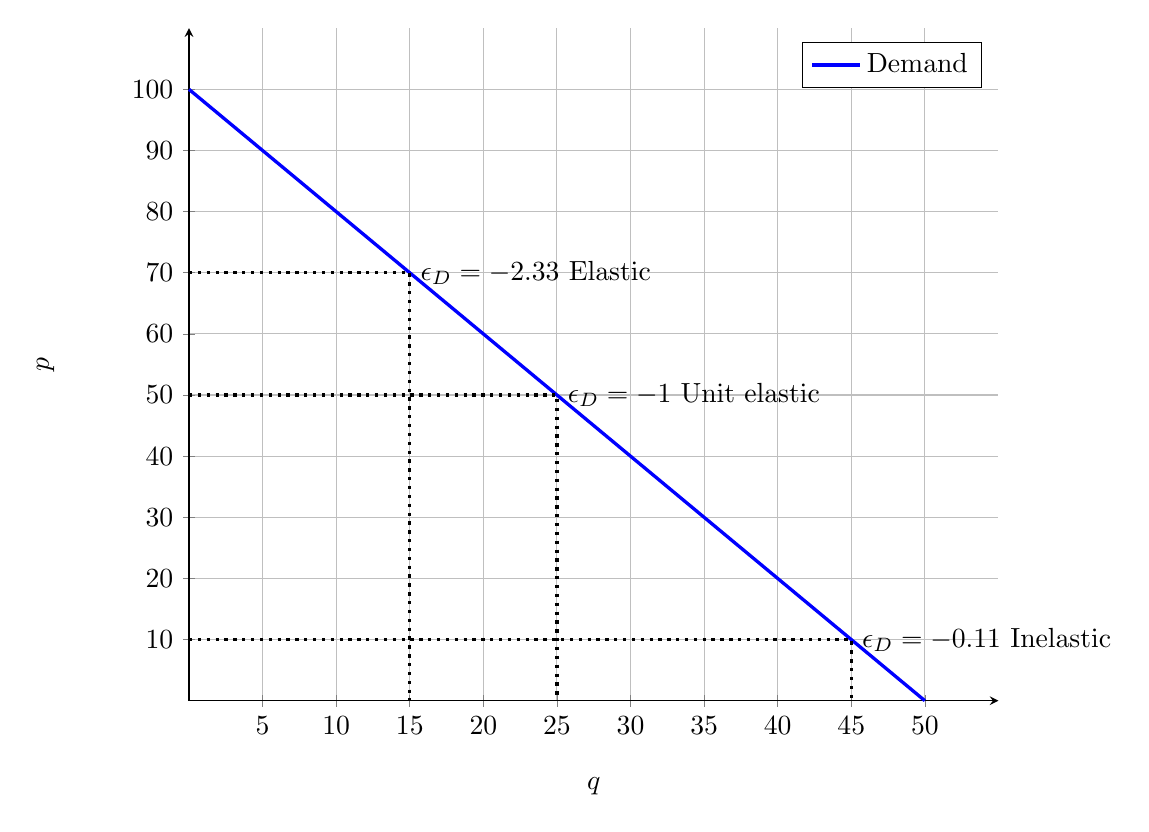
\begin{tikzpicture}
 			\begin{axis}[clip=false,
 			scale=1.5,
		axis lines=middle, 
		enlarge x limits={rel=0.1, upper},
		enlarge y limits={rel=0.1, upper},
		every axis y label/.style={at={(axis description cs:-0.2,0.5)},rotate=90,anchor=north},
		every axis x label/.style={at={(axis description cs:0.5,-0.1)},anchor=north},
	%legend pos=outer north east,
	xlabel=$q$,
	ylabel=$p$,
	shader=flat,
	xtick={0,5,...,50},
	ytick={0,10,...,100},
	grid=major,
	ymin=0,
	xmin=0,
	ymax=100,
	xmax=50,
]
	\addplot[domain=0:50, samples=25, very thick, color=blue]{100-2*x};
	\addlegendentry{Demand}
	\draw[black, very thick, dotted] (axis cs:0,70)--(axis cs:15,70)node[right]{$\epsilon_D=-2.33$ Elastic}--(axis cs:15,0);
	\draw[black, very thick, dotted] (axis cs:0,10)--(axis cs:45,10)node[right]{$\epsilon_D=-0.11$  Inelastic}--(axis cs:45,0);
	\draw[black, very thick, dotted] (axis cs:0,50)--(axis cs:25,50)node[right]{$\epsilon_D=-1$ Unit elastic}--(axis cs:25,0);
	\end{axis}
 	\end{tikzpicture}
	\end{center}

\end{document}